% Chapter 3: Methodology

Having covered the importance of LLM optimization and the technical architecture of Transformers in previous chapters, we now turn to the practical challenge of model compression.

The following sections begin with details on the preliminary experiments that revealed crucial insights about architectural redundancy in Transformer models and shaped the main compression strategy. It then presents what is possibly the heart of this research: a multi-stage pipeline that combines several optimization techniques in a structured sequence. Each stage is examined with both theoretical foundations and key implementation considerations. Finally, the evaluation framework is outlined along with the chosen metrics and benchmarks.

\section{Preliminary Research: Franken-LLaMA} \label{frankenllama}

Before embarking on systematic compression techniques for our target 1B parameter LLaMA model, preliminary research was conducted to understand the behavior of Transformer architectures under structural changes. This exploratory phase consisted on the ``Franken-LLaMA'' project \cite{franken-llama}, which involved experimenting with architectural modifications on the larger LLaMA2-7B-Chat model \cite{llama2} to gain a first insight into which components of the Transformer architecture are most critical for maintaining model performance.

The approach centered on modifying the standard Transformer execution flow by selectively including, excluding, or repeating attention blocks within the 32-layer architecture. Implementation was carried out using PyTorch \cite{pytorch}, with modifications to Hugging Face's transformers library \cite{hf_transformers} to enable dynamic layer skipping and repetition at runtime. The repetition strategy was particularly attractive as it could theoretically reduce memory footprint by reusing the same layer weights multiple times rather than storing distinct parameters for each position, and aligned directly with the target hardware constraints outlined in Section \ref{target_hardware}.

25 different layer configurations were tested, each of which was evaluated through qualitative text generation tasks and quantitative assessment on the HellaSwag dataset \cite{hellaswag}.
The results revealed that conservative modifications often maintained reasonable performance while reducing computational overhead. In particular, skipping layers towards the middle-end of the model rather than the beginning or final layers resulted in lower output quality degradation. For instance, the configuration that skipped layers 23 to 27 achieved a HellaSwag score of 0.38 compared to the baseline's 0.34 (the baseline consisted on the unmodified LLaMA 2 model), suggesting that certain middle layers may contribute less to final performance than expected.

However, more aggressive modifications typically led to a much more severe degradation in output quality. Configurations involving extensive layer repetition or using only sparse layer selections often produced incoherent text with non-ASCII characters and semantic breakdown. This behavior indicated that while some redundancy exists in the Transformer architecture, there are clear limits to how extensively the model can be modified before fundamental language capabilities deteriorate.

Results from this exploratory phase informed the subsequent approach to systematic compression, as they revealed that strategic layer removal could maintain acceptable quality levels while reducing computational overhead, suggesting that pruning techniques might offer promising avenues for optimization. At the same time, Franken-LLaMA proved that layer repetition was not a viable strategy and caused heavy performance degradation.

\section{An Overview of the Pipeline}

The core result of this research is the compression pipeline, which implements a sequential approach that combines multiple optimization techniques in a carefully orchestrated manner. As previously mentioned, the target model for these optimizations is LLaMA 3.2 1B, a distilled version of the larger LLaMA 3.2 model that has already undergone some level of pruning during its creation, according to the model documentation on Hugging Face \cite{llama3_1b}.

The choice of this particular model as the starting point is both strategic and practical. While incorporating distillation directly into the pipeline would have been ideal given its effectiveness as a compression technique \cite{homodistil}, the computational requirements make it rather prohibitive: in terms of complexity, distillation is essentially equivalent to training a model from scratch, thus requiring extensive GPU resources that far exceed the computational budget available for the project. In light of this, an existing pre-distilled model was utilized instead which already provides a rather compact foundation.

Following the approach established in the preliminary experiments (Section \ref{frankenllama}), the pipeline is implemented using PyTorch \cite{pytorch} for model modifications and Hugging Face's transformers library \cite{hf_transformers} for model loading and inference. The majority of configurations were developed using the Instruct version of LLaMA 3.2 1B \cite{llama3_1b_instruct}, as these instruction-tuned models are specifically optimized for dialogue and question-answering tasks that constitute the primary evaluation benchmarks in this work (see Section \ref{evaluation}), thereby minimizing the need for additional prompt engineering during testing phases. Nevertheless, the compatibility with the original model is kept, and the framework can produce configurations built upon the vanilla LLaMA 3.2 1B variant \cite{llama3_1b} by specifying a flag before execution.

The compression pipeline follows a five-stage progression, with each stage building upon the previous one. This particular ordering was chosen based on the complementary nature of these techniques and their relative impact on model structure.

\begin{enumerate}
    \item The first stage implements \textbf{depth-wise pruning} (Section \ref{depth_pruning}), where entire Transformer layers are removed based on importance metrics computed during a calibration phase. This coarse-grained approach eliminates redundant blocks, and ultimately redefines the skeleton of the architecture.

    \item \textbf{Width-wise pruning} follows as the second stage (Section \ref{wanda}), applying the WANDA algorithm \cite{wanda} to remove less critical weights within the remaining layers. This is a finer-grained approach compared to depth pruning, as it operates at the parameter level.

    \item The third stage introduces \textbf{\textit{Low-Rank Adaptation}} (LoRA) \cite{lora} (Section \ref{lora}) to recover performance lost during the pruning phases, while also allowing for fine-tuning on specific downstream tasks.

    \item The fourth stage applies 4-bit  \textbf{quantization} using GPTQ \cite{gptq_quantization} (Section \ref{quantization}), reducing the memory footprint of individual parameters.

    \item The final stage produces and applies an \textbf{\textit{Eigenspace Low-Rank Approximation}} (EoRA) \cite{eora} adapter (Section \ref{eora}) step to improve the performance of the quantized model.
\end{enumerate}

Detailed descriptions of each stage are provided in the following sections. Each step yields an intermediate model suitable for independent evaluation, except when the user specifies otherwise. Additionally, the pipeline features a comprehensive set of tuning options, such as the ability to skip specific stages or experiment with different parameter configurations without modifying the core implementation. This allows to conduct ablation studies more easily and adapt the framework to specific hardware constraints.

\section{Pruning Techniques} \label{pruning}

Pruning reduces neural network complexity by removing components according to importance criteria. The technique operates through two distinct main approaches that differ in their granularity and organization:

\begin{itemize}
    \item \textbf{Unstructured pruning} eliminates individual weights throughout the network randomly or based on an importance criteria such as magnitude.
    \item \textbf{Structured pruning} removes entire architectural units such as groups of neurons, attention heads, or complete layers.
\end{itemize}
Additionally, they can be further categorized based on the spatial dimension of the operation. In particular:
\begin{itemize}
    \item \textbf{Width pruning} targets components within layers, such as individual neurons inside an attention block.
    \item \textbf{Depth pruning} eliminates entire layers or Transformer blocks from the architecture. It is generally regarded as a form of structured pruning.
\end{itemize}
A visual comparison between these two pruning techniques is shown in Figure \ref{fig:pruning_comparison}.

\begin{figure}[htbp]
    \centering
    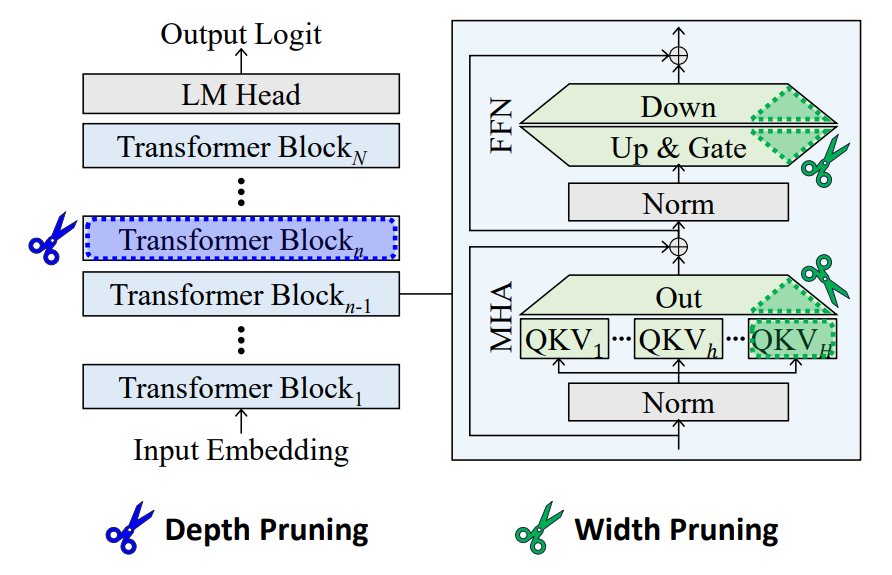
\includegraphics[width=0.7\textwidth]{pruning.png}
    \caption[Comparison of Depth and Width Pruning]{Depth pruning removes the single Transformer layers (left), while width pruning removes single neurons from the weight matrices (right). The image was retrieved from \cite{shortened_llama}.}
    \label{fig:pruning_comparison}
\end{figure}

\subsection{Depth Pruning} \label{depth_pruning}

Regarding depth pruning, the approach used in this project eliminates entire attention blocks following the methodology established by Kim et al. in their Shortened LLaMA work \cite{shortened_llama}, in which they define three metrics to determine the importance of a Transformer block:

\begin{itemize}
   \item \textbf{Magnitude-based importance}: computes L1 norms of weights within each block, assuming that layers with larger weight magnitudes contribute more significantly to model output.
   
   \item \textbf{Taylor expansion importance}: leverages gradient information to estimate removal impact through the approximation 
   \begin{equation}
    L(W = 0) \approx L(W) + \nabla L \cdot (-W)
   \end{equation}
   where the gradient-weight product indicates layer significance based on how loss would change if the layer were removed.
   
   \item \textbf{Perplexity-based importance}: temporarily removes each layer and measures performance degradation on calibration data through perplexity \cite{perplexity}, providing a direct empirical assessment of layer contribution to model quality (details on this metric are further explained in Section \ref{evaluation}).
\end{itemize}

While the pipeline implementation incorporates all three importance ranking methods, in practice, perplexity served as the main importance metric during testing due to its direct correlation with model performance degradation. In view of this, all layers are ranked according to their computed importance scores, with layers receiving lower rankings considered less critical and prioritized for removal during the pruning process.

Following insights from prior work in Section \ref{frankenllama} and Shortened-LLaMA \cite{shortened_llama}, the implementation protects the first four and last two layers from removal, as these positions prove critical for maintaining performance.

The pruning implementation creates a new model architecture with reduced depth by systematically copying weights from the original model while skipping the least important layers. The process begins by modifying the model configuration to reflect the reduced number of layers, then establishes a mapping between original and pruned layer indices. This mapping accounts for the gaps created by removed layers, ensuring that retained layers maintain their relative positioning and connectivity.

The resulting pruned model maintains the same computational pattern as the original but with fewer sequential operations, directly reducing inference latency and, most importantly, memory requirements.

\subsection{Width Pruning} \label{wanda}

The width pruning approach in this pipeline exclusively employs structured pruning techniques to maintain compatibility with modern hardware accelerators. Specifically, the implementation targets structured sparsity patterns supported by NVIDIA's sparse Tensor Cores in Ampere and Hopper architectures \cite{nvidia-width}. This sparsity pattern enables theoretical 2$\times$ compute throughput compared to dense matrix multiplication while maintaining efficient memory access. In particular, unlike unstructured pruning that creates irregular sparse matrices, structured sparsity preserves regular patterns that can be compressed when loaded into VRAM, storing only non-zero values and compact index metadata while mapping directly to accelerator capabilities without additional software overhead. A visual representation of the advantage is shown in Figure \ref{fig:nvidia-width}.

\begin{figure}[htbp]
    \centering
    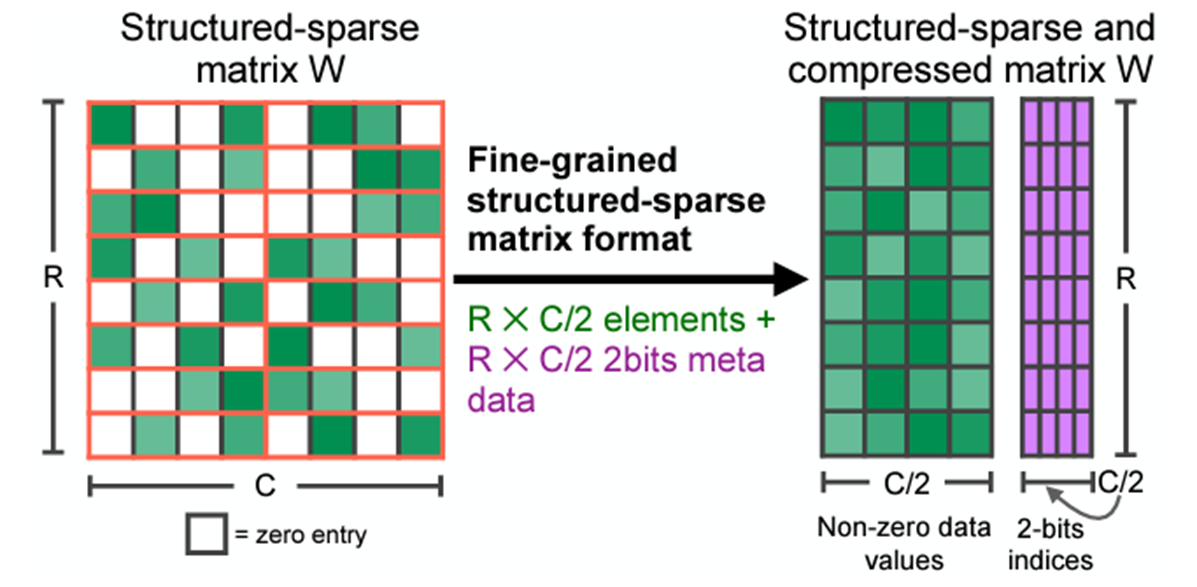
\includegraphics[width=0.7\textwidth]{structured-sparsity-pattern.png}
    \caption[Advantages of Structured Sparsity]{Visual representation of how the structured-sparse matrices are processed in NVIDIA's Ampere and Hopper GPUs. The image was sourced from \cite{nvidia-width}.}
    \label{fig:nvidia-width}
\end{figure}

\textit{Weight AND Activation-based pruning} (WANDA) \cite{wanda} serves as the core algorithm for implementing this structured approach. Originally developed for unstructured weight removal, WANDA's official implementation includes extensions for structured pruning patterns that align with the hardware requirements. The method leverages the observation that large language models develop outlier activations, which are emergent features with magnitudes significantly larger than typical hidden state values and are crucial for performance. Consequently, the WANDA importance metric for each weight $W_{ij}$ is defined as

\begin{equation}
S_{ij} = |W_{ij}| \cdot \|X_j\|_2
\end{equation}

where $|W_{ij}|$ represents the absolute weight magnitude and $\|X_j\|_2$ evaluates the L2 norm of the $j$-th input feature across calibration samples. This formulation addresses a key limitation of traditional magnitude-based importance, which is typically used by width pruning approaches, by accounting for input activations, which play an equally important role in determining neuron outputs.

The structured pruning process each layer by organizing weights into groups of $M$ consecutive elements (i.e. consecutive columns of the same row of the weight matrix) and removing the $N$ weights with lowest importance scores while retaining the rest. This is applied comprehensively to all linear layers in the Transformer architecture, including both the feed-forward networks and the attention-related projection matrices $W_Q$, $W_K$, $W_V$, and $W_O$ (see Section \ref{attention}). The activation statistics are collected by forward hooks during calibration, with each linear layer wrapped to compute the L2 norm of input activations across samples. After computing importance scores for each weight group, the implementation uses PyTorch's scatter operations to efficiently mark low-importance weights for removal. The algorithm completes pruning in a single forward pass using the C4 corpus \cite{c4} as calibration dataset.

\section{Low-Rank Adaptation (LoRA)} \label{lora}

\textit{Low-Rank Adaptation} (LoRA) \cite{lora} represents a parameter-efficient fine-tuning technique that addresses the computational and memory constraints associated with full model retraining. Rather than updating all model parameters during adaptation, LoRA introduces trainable low-rank decomposition matrices that capture the essential changes needed for task-specific performance. Figure \ref{fig:lora} provides an overview of this process.

\begin{figure}[htbp]
    \centering
    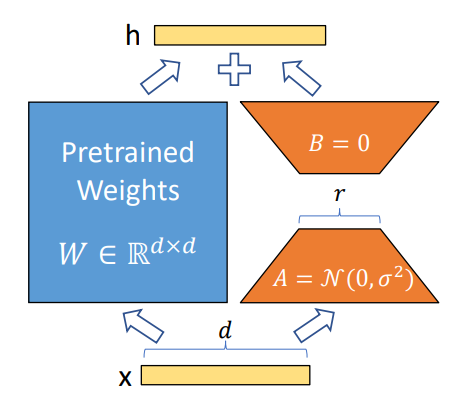
\includegraphics[width=0.4\textwidth]{lora.png}
    \caption[LoRA Overview]{A summary of the LoRA training process. We can see how the original pre-trained weights and the low-rank adapter are summed when the output activation is computed. The image was retrieved from the original LoRA paper \cite{lora}.}
    \label{fig:lora}
\end{figure}

The fundamental insight behind LoRA stems from the hypothesis that weight updates during adaptation have a low intrinsic rank, even when the full rank of the weight matrices is very high. For a pre-trained weight matrix $W_0 \in \mathbb{R}^{d \times k}$, LoRA constrains the update by representing it through a low-rank decomposition:

\begin{equation}
W_0 + \Delta W = W_0 + BA
\end{equation}

where $B \in \mathbb{R}^{d \times r}$, $A \in \mathbb{R}^{r \times k}$, and the rank $r \ll \min(d,k)$. During training, $W_0$ remains frozen while only $A$ and $B$ contain trainable parameters.

Consequently, the modified forward pass becomes:
\begin{equation}
h = W_0X + \Delta WX = W_0X + BAX
\end{equation}

The matrices are initialized such that $A$ follows a random Gaussian distribution while $B$ is initialized to zero, ensuring that $\Delta W = BA$ starts at zero so that the model begins with its original pre-trained behavior.

LoRA offers substantial reductions in trainable parameters while maintaining comparable performance to full fine-tuning. Its linear design allows to merge the low-rank matrices with frozen weights during deployment, introducing no additional inference latency. According to the original paper \cite{lora}, in Transformer architectures LoRA is most effective when applied to attention weights, particularly the query and value projection matrices ($W_q$ and $W_v$), with very low ranks ($r=1$ or $r=2$) often proving sufficient for downstream tasks.

Within the compression pipeline, LoRA serves as the third stage, following the pruning phases. This positioning is strategic: LoRA helps recover performance degraded by the aggressive structural modifications while simultaneously adapting the model for specific downstream tasks.

The implementation utilizes Hugging Face's \textit{Parameter-Efficient Fine-Tuning} (PEFT) library \cite{peft}, which provides optimized LoRA integration with Hugging Face's transformer models. The configuration specifically targets the four attention projection matrices: query ($W_Q$), key ($W_K$), value ($W_V$), and output ($W_O$) projections (see Section~\ref{attention}) with a rank of 8 and dropout rate of 0.1. Training employs mixed-precision optimization with gradient accumulation to maintain computational efficiency while adapting to the reduced parameter space.

\section{Quantization} \label{quantization}

Quantization represents a fundamental compression technique that maps continuous floating-point values to a discrete, finite set of representations, typically using low precision formats such as 8-bit or 4-bit integers. This approach is widely used on architectures such as Convolutional Neural Networks \cite{quant_cnn}, as these models are often deployed on edge devices and quantization offers a substantial memory reduction with controlled impact performance.

The quantization process follows the mapping:
\begin{equation}
\text{quant}(x) = \text{round}\left(\frac{x - z}{s}\right)
\end{equation}
where $x$ represents the original floating-point value, $s$ denotes the scale factor and $z$ is the zero-point offset. Subtracting the offset and dividing by the scale normalizes the floating-point value to the quantization grid, so that it is accurately represented within the discrete range of the target precision format.

However, this straightforward round-to-nearest approach often results in significant accuracy degradation. The GPTQ technique proposed by Frantar et al. \cite{gptq_quantization} addresses these limitations through a sophisticated post-training quantization algorithm that leverages second-order information from the Hessian matrix of the layer's reconstruction error to minimize quantization impact. Building upon the \textit{Optimal Brain Quantization} (OBQ) framework \cite{obq}, GPTQ formulates quantization as a layer-wise optimization problem where for each linear layer with weight matrix $W$ and calibration inputs $X$, the algorithm seeks quantized weights $\hat{W}$ that minimize the reconstruction error:
\begin{equation}
\arg\min_{\hat{W}} ||WX - \hat{W}X||_2^2
\end{equation}

The core innovation of GPTQ lies in its three-step algorithmic approach that enables scalability to billion-parameter models.

The first step is based on the idea that arbitrary quantization order suffices. Unlike OBQ, which greedily selects weights based on quantization error, GPTQ demonstrates that quantizing weights in any fixed order yields comparable results for large, heavily-parametrized layers. This insight allows all rows of the weight matrix to be quantized in the same column order, reducing the overall computational complexity.

The second step consists on the implementation of lazy batch updates. To address memory bandwidth bottlenecks, GPTQ processes weights in blocks of $B=128$ columns simultaneously. The algorithm exploits the observation that quantization decisions for column $i$ are only affected by updates to that specific column, enabling ``lazy batching" where updates are accumulated within blocks before global application:
\begin{equation}
\delta_F = -(w_Q - \text{quant}(w_Q))([H_F^{-1}]_{QQ})^{-1}(H_F^{-1})_{:,Q}
\end{equation}
\begin{equation}
H_{-Q}^{-1} = \left[H^{-1} - H_{:,Q}^{-1}([H^{-1}]_{QQ})^{-1}H_{Q,:}^{-1}\right]_{-Q}
\end{equation}
where $Q$ denotes the set of quantized weight indices within the current block, $F$ represents remaining full-precision weights, $w_q$ denotes a weight $\in Q$, $\delta_F$ is the compensation update applied to unquantized weights to minimize reconstruction error, and $H_{-Q}^{-1}$ is the updated inverse Hessian matrix with rows and columns corresponding to quantized weights $Q$ removed.

The final step is the Cholesky reformulation. For numerical stability at scale, GPTQ precomputes Hessian inverse information using Cholesky decomposition rather than iterative matrix updates. The Hessian matrix is computed as:
\begin{equation}
H = 2XX^T + \lambda I
\end{equation}
where $\lambda$ represents a damping factor (1\% of average diagonal value) for numerical stability. The Cholesky decomposition $H^{-1} = LL^T$ provides numerically stable access to required matrix rows while avoiding the accumulation of errors from repeated matrix inversions that plagued the older approaches when applied to large models.

The quantization procedure processes each layer independently, iterating through weight columns while maintaining compensation updates to remaining unquantized weights, and is applied to the attention matrices and linear layers of the Transformer.

The compression pipeline places quantization as the fourth stage, applied after pruning and LoRA adaptation phases, to strategically leverage the reduced parameter count from pruning. For the practical implementation, the GPTQModel toolkit \cite{gptqmodel} was employed, which provides optimized implementations of the GPTQ algorithm with support for various model architectures and quantization configurations. This toolkit handles the complex numerical computations and memory management required for large-scale quantization, allowing focus on the integration aspects within the broader compression pipeline. The quantization process utilizes 4-bit precision with a group size of 128, which means that groups of 128 consecutive weights share the same quantization parameters (scale and zero-point).

\subsection{Eigenspace Low-Rank Approximation (EoRA)} \label{eora}

Following quantization, \textit{Eigenspace Low-Rank Approximation} (EoRA) \cite{eora} can be optionally applied to recover accuracy lost during compression. EoRA is a rather novel technique which provides a training-free method to enhance performance of compressed models through low-rank matrix compensation by projecting compression errors into task-specific eigenspaces. Figure \ref{fig:eora} summarises the process in a schematic way.


\begin{figure}[htbp]
    \centering
    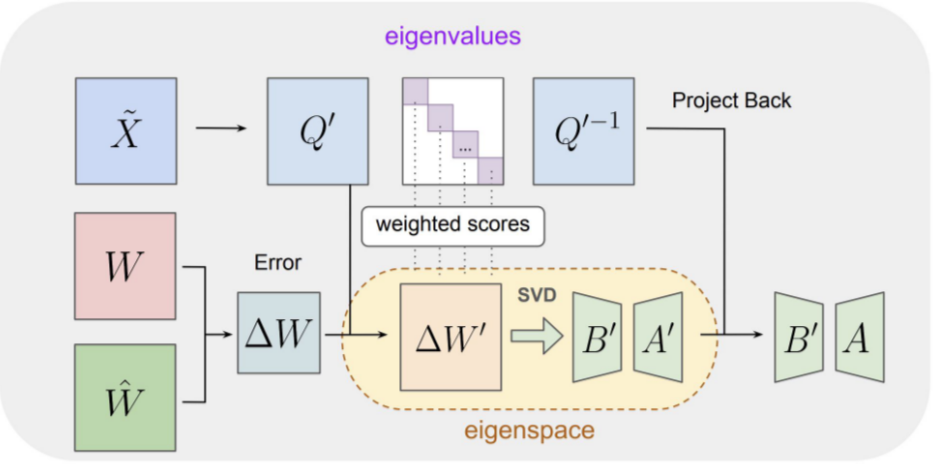
\includegraphics[width=0.7\textwidth]{eora.png}
    \caption[EoRA Overview]{The image summarizes the EoRA process in a schematic way, courtesy of \cite{eora}.}
    \label{fig:eora}
\end{figure}


Despite their similar names, EoRA differs fundamentally from Low-Rank Adaptation. While LoRA adapts pre-trained models to new tasks through gradient-based optimization of low-rank matrices, EoRA focuses on compensating compression-induced errors without training. Nevertheless, both methods employ additive low-rank corrections to weight matrices which are formulated as adapters.

As noted earlier, EoRA projects compression error into the eigenspace of layer-wise input activations before applying singular value decomposition. For a layer with original weights $W$ and compressed weights $\hat{W}$, compression error is $\Delta W = W - \hat{W}$. Rather than directly decomposing this error, EoRA first computes the eigendecomposition $\tilde{X}\tilde{X}^T = Q\Lambda Q^T$, where $\tilde{X}$ represents average input activations over the calibration dataset. This is done in order to derive the eigenspace projection matrix $Q$, whose columns are the eigenvectors, and $\Lambda$, which is a diagonal matrix containing the corresponding eigenvalues.

The projection of the compression error into the eigenspace is then computed using the transformation matrix $Q' = Q\sqrt{\Lambda}$:
\begin{equation}
\Delta W' = \Delta W \cdot Q'
\end{equation}

This eigenspace projection amplifies compression errors along directions of high activation variance (i.e. high eigenvalues) while diminishing those along low-variance directions, causing the subsequent SVD operation to naturally allocate more of its limited representational capacity to approximating the amplified, task-relevant error components.

Finally, the projected error $\Delta W'$ is decomposed using SVD to obtain $\Delta W' \approx B'A'$, where $B'$ and $A'$ are low-rank matrices. The final compensation matrices are obtained by back-projecting to the original space: $A = A'(Q')^{-1}$.

Similarly to LoRA, the forward pass on the compensated model becomes:
\begin{equation}
h = \hat{W}X + \Delta W'(Q')^{-1}X = \hat{W}X + B'A'(Q')^{-1}X = \hat{W}X + B'AX
\end{equation}

Implementation utilizes the GPTQModel toolkit \cite{gptqmodel}, which integrates EoRA compensation with existing quantized models. In the default configuration of the pipeline, the EoRA calibration step uses 64 samples from the C4 dataset \cite{c4}. This minimal calibration requirement represents one of the key advantages of this approach. Additionally, the adapter is generated using a rank of 32. Although the original paper employed a rank of 128 \cite{eora}, the GPTQModel documentation indicates that larger ranks can cause overfitting while obviously consuming more memory \cite{gptqmodel}. This issue may be particularly pronounced for smaller 1B models such as the one adopted in this work.


\section{Evaluation} \label{evaluation}

The evaluation system employs two distinct benchmarking datasets to assess model performance across different dimensions of language understanding. WikiText-2 \cite{wikitext} serves as the primary benchmark for measuring language modeling capability through perplexity computation \cite{perplexity}, while TriviaQA \cite{triviaqa} evaluates both reading comprehension and factual knowledge through question-answering tasks.

The implementation leverages a custom evaluation framework which automatically detects model types and applies appropriate loading procedures.

\subsection{WikiText-2 Perplexity Evaluation}

WikiText-2 \cite{wikitext} represents a collection of high-quality Wikipedia articles that serves as a standard benchmark for language modeling tasks. The dataset consists of over 2 million tokens extracted from verified Wikipedia articles, providing a diverse corpus of well-structured text that spans multiple domains and writing styles.

Perplexity serves as the fundamental metric for language model evaluation, measuring how well a model predicts the next token in a sequence. Mathematically, perplexity is defined as the exponential of the cross-entropy loss:

\begin{equation}
\text{Perplexity} = \exp\left(\frac{1}{N} \sum_{i=1}^{N} -\log P(w_i | w_1, w_2, \ldots, w_{i-1})\right)
\end{equation}

where $N$ represents the total number of tokens, $w_i$ denotes the $i$-th token, and $P(w_i | w_1, w_2, \ldots, w_{i-1})$ represents the model's predicted probability for the correct next token given the preceding context.
Lower perplexity values indicate better language modeling performance, with the metric providing intuitive interpretation: a perplexity of $X$ means the model is, on average, as confused as if it had to choose uniformly among $X$ possibilities for each token.

The evaluation protocol processes the whole WikiText-2 test split (trimmed to 512 sequence length) by accumulating negative log-likelihoods across all valid tokens before computing the final exponential transformation. The implementation iterates through sequences, computing cross-entropy loss for each token while applying attention masks to exclude padding tokens from the calculation, ensuring that only meaningful content contributes to the perplexity measurement.

\subsection{TriviaQA Question-Answering Evaluation}

TriviaQA \cite{triviaqa} constitutes a comprehensive reading comprehension dataset containing over 650,000 question-answer pairs sourced from trivia and quiz-bowl competitions. The dataset's distinctive characteristic lies in its dual-mode evaluation framework that enables assessment of both knowledge retrieval and reading comprehension capabilities through closed-book and open-book testing scenarios.

The closed-book evaluation presents models with questions in isolation, requiring them to rely entirely on knowledge encoded in their parameters during training. This mode directly tests the factual knowledge retention of compressed models and reveals whether compression techniques have degraded the model's ability to recall specific information. Questions use a simple prompt structure: ``Question: [question text] Answer:''.

Conversely, the open-book evaluation provides relevant context passages alongside each question, which simulates a reading comprehension scenario where models must extract answers from provided text. The context is derived from TriviaQA's associated search results, with the implementation selecting the shortest available context passage to minimize computational overhead while preserving essential information. Consequently, the prompt format becomes: ``Context: [context passage] Question: [question text] Answer:''.

Answer correctness evaluation employs a three-tier verification system designed to accommodate the variability inherent in natural language responses. The evaluation process begins with testing the exact matching of the answer, where the generated text is compared directly against all provided correct answer aliases after normalization. Normalization involves converting text to lowercase, removing punctuation, and standardizing whitespace to ensure fair comparison despite minor formatting differences.

When exact matching fails, the system applies substring matching, checking whether any correct answer appears as a contiguous substring within the generated response. This approach accounts for models that provide correct answers embedded within longer explanations or additional context, which is common behavior in instruction-tuned models.

The final verification stage implements fuzzy matching for cases where neither exact nor substring matching succeeds. For answers containing multiple words, the system computes the intersection between the set of words in the generated answer and each correct answer, considering a response correct if at least 80\% of the words in the target answer appear in the generated text:

\begin{equation}
\text{Fuzzy Match} = \frac{|\text{Words}_{\text{generated}} \cap \text{Words}_{\text{correct}}|}{|\text{Words}_{\text{correct}}|} \geq 0.8
\end{equation}

Generation parameters are carefully set up to ensure consistent evaluation conditions. Models generate between 1 and 50 tokens per answer using deterministic decoding (with temperature set to 1.0) to mitigate randomness that could affect reproducibility. The evaluation framework processes 1200 samples of TriviaQA's validation split (alternatively, the quantity of samples can be tuned by the user), and the accuracy is computed separately for these two tasks.